\chapter{More About Configuring MATSim}
\label{ch:configuring}
% ##################################################################################################################

\hfill \textbf{Author:} Andreas Horni, Kai Nagel

\begin{center} 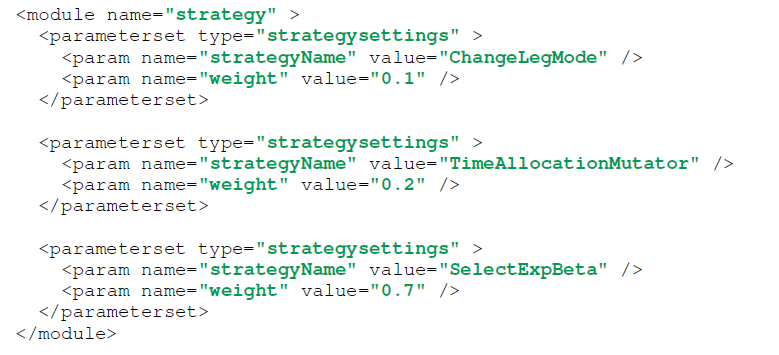
\includegraphics[width=0.3\textwidth, angle=0]{using/figures/strategy.png} \end{center}

% ##################################################################################################################
In this chapter, configuration options are described that are exclusively done by the \gls{configfile}. \gls{matsim} configuring  requiring further input data beyond the three basic elements---\ie the \gls{configfile}, a population and a network---are described in Chapter~\ref{ch:modules}. The technical details for module usage, in particular the parameter sets are described in \citep[][]{MATSim_Userguide_2015} and in the \gls{javadoc}.

% ##################################################################################################################
\section{MATSim Data Containers}
\label{sec:using-data-containers}
\kai{Eigentlich steht das alles schon in Section~\ref{sec:inputdata}.  Ist es wirklich sinnvoll, das zu doppeln?  Oder schreiben wir hier halt die ``weiteren'' Container rein (dann sollten wir aber einiges weitere von oben hier runter holen).}
\ah{M.E. jetzt ok.}

% ===================================================================================
\subsection{Network}
\label{sec:using-network}
The \gls{configfile} section \lstinline|network| amongst other specifies which network file will be used in the simulation (Section~\ref{sec:lgs-config} and \ref{sec:lgstarted-network-file}). Further configuration options, \eg specification of time-variant networks, are presented in Section~\ref{sec:extending-network}.

% ===================================================================================
\subsection{Population}
\label{sec:using-population}
The \gls{configfile} section \lstinline|plans| allows to specify the population with its day plans (Section~\ref{sec:lgs-config} and \ref{sec:lgstarted-population-file}). Further configuration options, \eg specification of arbitrary agent attributes or subpopulations, are presented in Section~\ref{sec:extending-population}.

Further \gls{matsim} containers are described in Section~\ref{sec:extending-data-containers}.

%##################################################################################################################
\section{Global Modules and Global Aspects}
\label{sec:using-globalmodules}
% ===================================================================================
\subsection{Controler}
\label{sec:using-controler}
The controler is an indispensable module for running \gls{matsim}, its parameters are set in the \lstinline|controler| \gls{configfile} section. Besides others, the \gls{matsimrun}'s output directory, its number of iterations, and the ouput interval of plans and events can be specified here. Also, the \gls{mobsim} to be used can be defined (Section~\ref{sec:using-mobsims}). Importantly, the routing algorithm is defined here by using
%
\begin{xml}
<module name="controler" >
    <param name="routingAlgorithmType" value="{Dijkstra | FastDijkstra |
    		AStarLandmarks | FastAStarLandmarks}" />
    [...]
</module>
\end{xml}
%
In Section~\ref{sec:extending-controler}, the possibilities to extend the \lstinline|Controler| functionality is given in Section~\ref{sec:extending-controler} and Chapter~\ref{ch:extensionpoints}.

% ===================================================================================
\subsection{Global}
\label{sec:using-global}
In the \gls{configfile} section \lstinline|global| the simulation's random seed, the number of \gls{java} threads assigned to the replanning modules, and the coordinate system to be applied (\cf Section~\ref{sec:unitsconventions}), can be defined. 
\kai{number of threads: nicht unter parallel computing?  Wäre meiner Erfahrung nach tatsächlich hilfreich, die paralellen Aspekte zusammenzufassen.} \ah{\url{https://matsim.atlassian.net/browse/MATSIM-310}}.

% ===================================================================================
\subsection{Parallel Event Handling}
\label{sec:using-paralleleventhandling}
The \gls{configfile} section \lstinline|parallelEventHandling| is used to define the number of threads used for event handling. 
As described in \citet[][]{WaraichEtAl_TechRep_IVT_2009, WaraichEtAl_STRC_2009} the simulation can be substantially speed-up when using multiple threads for the events handling, usually being a bottleneck in \gls{matsim} simulation runs.
% Clearly, the number of threads should correspond with available processor cores.  \kai{Meine Erfahrung ist eine andere, und je nach Maschine kann man das manchmal überauslasten und manchmal sollte man es eher unterauslasten.}  
According to our experiences the optimal degree of capacity utilization (threads versus cores) is highly machine-dependent.
As mentioned above, the \gls{mobsim} \gls{qsim} is running parallel by default.

Being able to speed-up scenarios might become even more important than today, when additional innovation (choice) dimensions are added with large variability in the parameters rendering ensemble runs necessary. % (see Section~\ref{sec:variability}).

%\ah{Marcel hatte mal Testreihe mit Identifikation der Laufzeit einzelner Module (QSim, Eventshandling etc.) geplant. Nachfragen, ob schon was vorhanden}

% ##################################################################################################################
\section{Mobility Simulations}
\label{sec:using-mobsims}
An overview of \gls{matsim} mobility simulations is given in \citet[][]{Dobler_TechRep_IVT_2011}. %See also the presentation of \citet[][]{Rieser_unpub_IVT_2011}.

% ===================================================================================
\subsection{\protect\gls{qsim}}
\label{sec:using-qsim}
The queue-based and time-step based \gls{qsim} \citep[][]{Dobler_TechRep_IVT_2011, Dobler_STRC_2010} is \gls{matsim}'s default \gls{mobsim}. Its parameters are set in the \lstinline|qsim| \gls{configfile} section. Prominent parameters are as follows. By specifying the parameter \lstinline|numberOfThreads| \gls{qsim} can be run in parallel. Importantly, this section's parameters \lstinline|flowCapacityFactor| and \lstinline|storageCapacityFactor| need to be set accordingly, when running sample scenarios, \eg for a 10\,\% sample, these factors need to be divided by 10. The \gls{matsim} \gls{gui} (Figure~\ref{fig:matsimgui}) allows to adapt these parameters with the command \lstinline|Tools...Create Sample Population|.

The link dynamics, either \gls{fifo} or passing can be specified by the parameter \lstinline|linkDynamics|. Back-propagating gaps (Section~\ref{sec:trafficflowmodel}) can be added with the parameter \lstinline|trafficDynamics|.

As shown in Section~\ref{sec:multimodalsim_qsim}, \gls{qsim} can handle \gls{multimodal} scenarios.

\ah{explizit hinzufügen ist jetzt nicht mehr nötig, weil default, oder?}
To invoke \gls{qsim}, the parameter \lstinline|mobsim| of \lstinline|controler| \gls{configfile} section must be set to \lstinline|qsim| and a \lstinline|qsim| \gls{configfile} section must be provided. 

% ===================================================================================
\subsection{JDEQSim}
\label{sec:using-jdeqsim}
\gls{jdeqsim} \citep[][]{WaraichEtAl_TechRep_IVT_2009, WaraichEtAl_STRC_2009} was used for project \emph{KTI Frequencies} \citep[][]{BalmerEtAl_ResRep_datapuls_2010}. It is is a \gls{java} reimplementation of \gls{deqsim} \citep[][]{WaraichEtAl_STRC_2009, CharyparEtAl_TRR_2007, CharyparEtAl_TRB_2009} and provides parallel event handling but no parallel simulation \citep[][p.11]{BalmerEtAl_ResRep_datapuls_2010}. Back-propagating gaps (Section~\ref{sec:trafficflowmodel}) are supported. Traffic lights, public transport and within-day replanning are not supported.

To run \gls{jdeqsim} the parameter \lstinline|mobsim| of \lstinline|controler| \gls{configfile} section must be set to \lstinline|JDEQSim| and a \lstinline|jdeqsim| \gls{configfile} section must be provided. 

%##################################################################################################################
\section{Scoring}
\label{sec:using-scoring}
The \gls{configfile} section \lstinline|planCalcScore| specifies the parameters used for scoring agents' plans (Section~\ref{sec:lgs-config}); parameters are explained in detail in the next chapter~\ref{ch:scoring}.

%##################################################################################################################
\section{Replanning Strategies}
\label{sec:strategymodules}
%\kai{Habe ``strategy'' ans Ende gezogen, weil ein matsim run so auch tatsächlich losgeht: erst mobsim, dann scoring, dann replanning.  Gibt es Argumente für andere Reihenfolgen?} \ah{nein, super Punkt!}
The replanning strategy modules are the basic innovation modules available in \gls{matsim}. We do not call them \emph{choice} modules although they are involved in people's choice making. The choice process, however, is performed over the iterations with an \emph{implicit} choice set and it is not based on explicit probability function drawing. Usually, innovation modules also do no define their own utility function. This is particularly true for random mutation modules, where best response modules such as destination innovation are closer to the standard procedure of choice modeling but still not full-blown choice models. For a detailed discussion of \gls{matsim} in choice modeling context see Chapter~\ref{ch:discretechoice}.

All strategy modules are called by configuring the strategy module in the configuration file as shown in the following example.
%
\begin{xml}
<module name="strategy" >
	<parameterset type="strategysettings" >
		<param name="strategyName" value="ChangeLegMode" />
		<param name="weight" value="0.1" />
	</parameterset>
	
	<parameterset type="strategysettings" >
		<param name="strategyName" value="TimeAllocationMutator" />
		<param name="weight" value="0.2" />
	</parameterset>
	
	<parameterset type="strategysettings" >
		<param name="strategyName" value="SelectExpBeta" />
		<param name="weight" value="0.7" />
	</parameterset>
</module>
\end{xml}
%
Each module is given a weight which determines the probability by which the course of action represented by the module is taken. The weights of the strategy modules are normalized in case they do not sum to one. In this example, each agent changes his leg mode with probability~0.1, its plan timing with probability 0.2. A strategy module is, in the code, always a combination of a plan selector and zero or more strategy module elements. In the example, the agent chooses a plan from his set of plans according to a logit model with probability~0.7. 

By specifying the parameter \lstinline|subpopulation|, replanning strategies can be applied to distinct sub-populations: \eg
\begin{xml}
	<parameterset type="strategysettings" >
		<param name="strategyName" value="ChangeLegMode" />
		<param name="weight" value="0.1" />
		<param name="subpopulation" value="urbanTravelers"/>
	</parameterset>
\end{xml}

In older versions of the \gls{configfile} you will find following deprecated configuration syntax using numbered strategy modules:
%
\begin{xml}
<module name="strategy" >
    <!-- NOTE: The following is deprecated syntax. -->
    <param name="ModuleProbability_1" value="0.1" /> 
    <param name="Module_1" value="ChangeLegMode" />
    <param name="ModuleProbability_2" value="0.2" />
    <param name="Module_2" value="TimeAllocationMutator" />
    <param name="ModuleProbability_3" value="0.7" />
    <param name="Module_3" value="SelectExpBeta" />
</module>
\end{xml}
%
%% \kai{Hier gibt es eine neue, bessere Syntax.  NB dass wir da gerade noch am ``Verhandeln'' sind!}
%% \ah{angepasst}
%
%% By specifying the parameter \lstinline{ModuleSubpopulation_X}, i.e.,
%% \begin{xml}
%%     <!-- NOTE: The following is deprecated syntax. -->
%%     <param name="ModuleSubpopulation_1" value="externalAgent"/>
%% \end{xml}
%% replanning strategies can be applied to distinct sub-populations.
%
% brauchen wir m.E. nicht. kai, jan'15


Please note, that combining strategy modules that are \glspl{contribution} such as destination innovation and public transport is not straight forward. Combine them with care and contact the mailing list in case you are unsure.

%Combining different modules is not straight-forward in MATSim. This important topic urgently awaits future analysis. To begin with, here, the combination of the strategy modules with public transport is presented in Table \ref{tab:combination}.
%
%% ----------------------------------
%\createtable%
%{Strategy Module Combination}%
%{Strategy Module Combination}%
%{\label{tab:combination}}%
%{%
  %\begin{tabular}[c]{|c|c|c|}
   %\hline
%\textbf{Innovation Dimension}	& \textbf{Default Strategy} & \textbf{Public Transport}\\
%\hline
%time innovation & TimeAllocationMutator &  TransitTimeAllocationMutator\\
%\hline
%route innovation & ReRoute & ReRoute \\
%\hline
%mode innovation & \multirow{2}{*}{ChangeLegMode} & \multirow{2}{*}{TransitChangeLegMode} \\
%(all legs get same mode) &  &  \\
%\hline
%mode innovation & \multirow{2}{*}{ChangeSingleLegMode} & \multirow{2}{*}{TransitChangeSingleLegMode} \\
%(each leg can have a different mode) &  &  \\
%\hline
%mode innovation & \multirow{2}{*}{SubtourModeChoice} & \multirow{2}{*}{TransitSubtourModeChoice} \\
%(subtour-based) &  &  \\
%\hline
%destination innovation & LocationChoice & LocationChoice \\
%\hline
  %\end{tabular}
%}%
%{}

%\kai{Ich meine, dass es diese Transit Sonderformen gar nicht mehr gibt.  ????}
%\ah{habs mal auskommentiert und die Warnung über Contrib-Kombinationen oben hingeschrieben.} 

% ===================================================================================
\subsection{Time Innovation}
\label{sec:timechoice}
Time innovation is applied by defining its parameters in the \gls{configfile} section \lstinline|TimeAllocationMutator| and by adding 
%
\begin{xml}
	<param name="strategyName" value="TimeAllocationMutator" />
\end{xml}
%
plus its weight to the strategy modules.

The module shifts activity end times randomly within a configurable range as described by \citet[][]{BalmerEtAl_Timmermans_2005, Raney_PhDThesis_2005, Balmer_unpub_VSP_2004, BalmerEtAl_unpub_EIRASS_2004, BalmerEtAl_unpub_STRC_2004}. %A best-reponse approach to time choice is applied by "Planomat" described in Section~\ref{sec:planomat}.

% ===================================================================================
\subsection{Route Innovation}
\label{sec:routechoice}

Route innovation is applied by defining its parameters in the \gls{configfile} section \lstinline|planscalcroute|, by adding 
%
\begin{xml}
	<param name="strategyName" value="ReRoute" />
\end{xml}
%
plus its weight to the strategy modules, and by specifying the routing algorithm in the \lstinline|controler| \gls{configfile} section (Section~\ref{sec:using-controler}).
\gls{matsim} routing is described by \citet[]{LefebvreBalmer_STRC_2007, LefebvreBalmer_TechRep_IVT_2007}. 

%The configuration necessary for public transport is shown in Chapter \ref{ch:pt}.  \kai{Da steht m.E.\ noch nichts in der Richtung.  Aber meiner Erinnerung nach ist auch gar keine Sonderkonfiguration mehr nötig.  Michael Z.?}
%
%\ah{Kann tatsächlich auch keine Sonderkonfiguration (mehr) finden unter \url{http://www.matsim.org/docs/tutorials/transit}. Kann man also wegmachen. Muss zu Config-Param "transitRouter" noch was gesagt werden?}

% ===================================================================================
\subsection{Mode Innovation}
\label{sec:modechoice}
Mode innovation is applied by adding 
%
\begin{xml}
	<param name="strategyName" value="{ChangeLegMode | ChangeSingleLegMode | SubtourModeChoice}" />
\end{xml}
%
plus its weight to the strategy modules. In the \gls{configfile} a section with one of the mode innovation strategies need to be added, \ie 
%
\begin{xml}
<module name="{changeLegMode | changeSingleLegMode | subtourModeChoice}" >
    [...]
</module>
\end{xml}
%\kai{obiges hat jetzt 2x ``changeLegMode''.  Kann zwar sein, dass das tatsächlich so ist, aber falls ja, sollten wir explizit sagen, dass das kein Tippfehler ist.} \ah{thx}
%
\lstinline|ChangeLegMode| randomly picks one of the plans of a person and changes its mode of transport. By default, the supported modes are driving a car and using public transport. Only one mode of transport per plan is supported. For using different modes for sub-tours on a single day the \lstinline|SubtourModeChoice| module is required. Optionally, car availability is respected. \lstinline|ChangeSingleLegMode| randomly picks one of the plans of a person and changes the mode of transport of one single leg. The leg is picked randomly. In contrast to \lstinline|ChangeLegMode|, it allows for multiple modes in one plan. By default, the supported modes are driving a car and using public transport. Also, this module is able to (optionally) respect car-availability.

Mode innovation is described by \citet[][]{RieserEtAl_TRR_2009, MeisterEtAl_WCTRS_2010, CiariEtAl_STRC_2008, CiariEtAl_STRC_2007}.

% ===================================================================================
\subsection{Selectors}
\label{sec:selectors}
Selectors and their weight are also added to the strategy modules
%
\begin{xml}
	<param name="strategyName" value="KeepLastSelected | BestScore | SelectExpBeta
					ChangeExpBeta | SelectRandom | SelectPathSizeLogit" />
\end{xml}
%
Selectors work as follows:
%
\begin{itemize}\styleItemize
	\item \lstinline|KeepLastSelected| keeps the plan selected in the previous iteration.
	\item \lstinline|BestScore| selects the plan with the highest score of the previous iteration.
	\item \lstinline|SelectExpBeta| performs \gls{mnl} selection between plans. It can be configured by the \lstinline|BrainExpBeta| parameter from the scoring group.
	\item \lstinline|ChangeExpBeta| changes to a different plan with probability dependent on $e^{\Delta_{score}}$, where $\Delta_{score}$ is the score difference between the two plans.
	\item \lstinline|SelectRandom| performs random selection between the plans.
	\item \lstinline|SelectPathSizeLogit| selects an existing plan according to the path size logit described by \citet[][]{FrejingerBierlaire_TransResB_2007}.
\end{itemize}
%
Note, that the \lstinline|BestScore| should be used with care as it is prone to getting stuck with sub-optimal plans. Plans that are rated bad due to a random fluctuation in one single iteration, due to \eg a rare traffic jam, will never be tested again. It is therefore recommended to use this in conjunction with \lstinline|SelectRandom| only.

Besides the selectors for plan modification and execution, in the near future also the plan remover will be available for configuration. Per default, the plan with the lowest score is removed if the agent's memory is full. In line with the requirements of \eg simulated annealing approaches, the removal of candidates will be configurable to be probabilistically dependent on the plan score similar to the selection in \lstinline|SelectExpBeta|. This will reduce the probability to get stuck with sub-optimal plans, that were dominant in earlier iterations.
%\ah{siehe Mail by M. Zilske, August 14 "[Matsim-devel] custom plan selector for removal")}

%##################################################################################################################
\section{Observational Modules}
\label{sec:observational}

% ===================================================================================
\subsection{Travel Time Calculator}
\label{sec:ttc}
The routing module, as an example, needs travel time estimations for all links of the network. To keep the computational effort feasible, the travel time estimations need to be aggregated to time bins. The parameters of this aggregation, such as the bin size, can be specified in the configuration file section \lstinline|travelTimeCalculator|.

% ===================================================================================
\subsection{Link Stats}
\label{sec:linkStats}
The \lstinline|linkStats| \gls{configfile} section allows to specify the output interval of simulation statistics of individual links. It is configurable, if the simulated volumes should be written per iteration or averaged over multiple iterations. Link stats are, amongst other, used for the comparison with count values as introduced in Section~\ref{sec:extending-counts}. 

% ##################################################################################################################
% Local Variables:
% mode: latex
% mode: reftex
% mode: visual-line
% TeX-master: "../main"
% comment-padding: 1
% fill-column: 9999
% End: 
